\subsection{Where RGB change falls}
\label{sec:v19-pixel}
For every native output and its source, let $\delta_p$ be the mean absolute difference of the three RGB channels in $[0,1]$. For $N$ pixels and the official edit mask $M_{\rm edit}$, define
\[
 \begin{aligned}
T&=N^{-1}\sum_p\delta_p, & F&=N^{-1}\sum_{p\in M_{\rm edit}}\delta_p,\\
B&=N^{-1}\sum_{p\notin M_{\rm edit}}\delta_p, & \rho&=F/T .
\end{aligned}
\]
$T$ is whole-image MAE. $F$ and $B$ express edit and background change per whole-image pixel, so $T=F+B$ and $B=T(1-\rho)$. Dividing $F$ by the edit-area fraction instead gives edit-region MAE. The per-output CSV also supplies mask areas, unnormalized masses $NF,NB$, and separate flags for an empty background or zero total change.

The 900 outputs comprise 18 configurations for each of 50 sources. Eight full edit masks account for 144 outputs. For these outputs $B=0$ and $\rho=1$, and the background-region scores are undefined. All 900 have positive total change and nonempty edit masks. The mean edit-area fraction is 0.3188 on the 42 sources with a background and 0.4278 on all 50. The 160 retained source-correction outputs cover 40 sources, two allocations at reference profile U, and seeds 0 and 17. All 160 have positive total change and both regions. We average the seeds within source before cohort summaries and paired bootstrap resampling.

\begin{table*}[t]
\centering\small
\caption{Mean RGB change on 42 background-eligible sources and on all 50. Each source carries equal weight. The alternate reference-profile runs appear below the default configurations.}
\label{tab:v19-pixel-levels}
\setlength{\tabcolsep}{4.0pt}
\begin{tabular}{lrrrrrrrr}
\toprule
&\multicolumn{4}{c}{42 with background}&\multicolumn{4}{c}{All 50}\\
\cmidrule(lr){2-5}\cmidrule(lr){6-9}
Configuration &$\bar T$&$\bar\rho$&$\bar F$&$\bar B$&$\bar T$&$\bar\rho$&$\bar F$&$\bar B$\\
\midrule
Spatial SAM & 0.0283 & 0.4798 & 0.0135 & 0.0148 & 0.0297 & 0.5631 & 0.0173 & 0.0124 \\
Uniform SAM & 0.0600 & 0.3795 & 0.0241 & 0.0359 & 0.0637 & 0.4788 & 0.0335 & 0.0302 \\
Two constants & 0.0344 & 0.3706 & 0.0127 & 0.0217 & 0.0359 & 0.4713 & 0.0176 & 0.0183 \\
FlowEdit (24) & 0.0602 & 0.3717 & 0.0225 & 0.0378 & 0.0637 & 0.4722 & 0.0320 & 0.0317 \\
\midrule
Uniform at S & 0.0343 & 0.3700 & 0.0126 & 0.0218 & 0.0357 & 0.4708 & 0.0174 & 0.0183 \\
Spatial at U & 0.0460 & 0.5201 & 0.0248 & 0.0212 & 0.0495 & 0.5969 & 0.0317 & 0.0178 \\
\bottomrule\end{tabular}\end{table*}

Figure~\ref{fig:v19-response-sensitivity}(c) places each configuration at $(\bar T,\rho_{\mathrm{mass}})$, where $\rho_{\mathrm{mass}}=\bar F/\bar T$. Its dashed curves satisfy $\bar B=\bar T(1-\rho_{\mathrm{mass}})$ exactly; their labels give mean background RGB mass per image pixel. In Table~\ref{tab:v19-pixel-levels}, $\bar\rho$ averages individual shares. For uniform SAM on 42 sources, $\bar B=0.03593$, while $\bar T(1-\bar\rho)=0.03721$. The difference is $-\operatorname{Cov}(T,\rho)$ using population normalization. The panel uses the shared 42-source cohort. Each of 10,000 bootstrap draws resamples the same source IDs across configurations (seed 0). A pointwise joint 95\% ellipse for each configuration uses the bootstrap covariance and the empirical 95th percentile of the bootstrap Mahalanobis distance from the observed point.

Compared with uniform on the 42 sources, two constants change whole-image MAE by $-0.02555$ [$-0.03037,-0.02128$] and the mean individual edit share by $-0.00890$ [$-0.01919,0.00023$]. For spatial SAM the corresponding differences are $-0.03170$ [$-0.03712,-0.02669$] and $+0.10032$ [$0.07016,0.13065$]. Against the constants, spatial SAM increases the share by $0.10922$ [$0.08099,0.13835$].

\paragraph{Background fidelity.}
We compute PSNR from mean squared RGB error on background pixels with unit data range, and SSIM channelwise using uniform $7\times7$ windows, sample variances and covariances, $C_1=0.01^2$ and $C_2=0.03^2$. Only windows fully contained in the image and in the background contribute. All 42 eligible sources have valid windows and finite PSNR in every configuration. Mean background PSNR/SSIM is 22.52/0.822 for uniform, 27.29/0.903 for two constants, 29.17/0.920 for spatial SAM and 21.91/0.795 for FlowEdit. Spatial minus constants is $+1.885$ dB [$1.146,2.667$] and $+0.01685$ SSIM [$0.01060,0.02368$].

\paragraph{Source correction at the uniform reference profile.}
The retained native-resolution outputs pair U25 with REQ-U. Uniform and spatial have mean $T$ of 0.11390 and 0.11340, mean individual $\rho$ of 0.36857 and 0.38402, and mean $B$ of 0.07260 and 0.07022. Spatial minus uniform changes mean $T$ by $-0.00049$ [$-0.00156,0.00052$], mean $\rho$ by $+0.01545$ [$0.00833,0.02277$], and mean $B$ by $-0.00238$ [$-0.00345,-0.00131$]. The mean edit-area fraction is 0.32378. Each interval resamples the 40 seed-averaged sources.

\subsection{Sensitivity to the matching coordinate}
Table~\ref{tab:v19-pixel-mrc} uses the study-wide preservation score: full-image spatial LPIPS averaged over the background. For each source, both five-setting curves must have complete finite points; we integrate on positive-width shared support, taking the first knob-ordered crossing and averaging the uniform-minus-spatial or FlowEdit-minus-SAM difference across that interval. Directional CLIP measures text response. Edit MAE measures local pixel-change magnitude; $\rho$ measures edit-region concentration. These two sensitivity coordinates are computed from the final pixels. Percentile intervals resample each pair's supported sources, equally weighted, 10,000 times with seed 0.

\begin{table*}[t]\centering\small
\caption{Harmonized preservation LPIPS at three matching coordinates. Positive differences favor the subtracted arm. Support and positive counts are source counts.}
\label{tab:v19-pixel-mrc}
\setlength{\tabcolsep}{5pt}
\begin{tabular}{llrrrr}
\toprule Coordinate & Comparison & Support & Mean [95\% CI] & Median & Positive\\\midrule
Directional CLIP & Uniform $-$ spatial & 41/42 & 0.0390 [0.0106, 0.0632] & 0.0271 & 37 \\
 & FlowEdit $-$ spatial & 38/42 & 0.1196 [0.0739, 0.1631] & 0.0953 & 35 \\
 & FlowEdit $-$ uniform & 41/42 & 0.0638 [0.0229, 0.1046] & 0.0622 & 32 \\
\midrule
Edit MAE & Uniform $-$ spatial & 42/42 & 0.0417 [0.0227, 0.0598] & 0.0394 & 37 \\
 & FlowEdit $-$ spatial & 41/42 & 0.0834 [0.0584, 0.1092] & 0.0813 & 37 \\
 & FlowEdit $-$ uniform & 42/42 & 0.0260 [0.0089, 0.0436] & 0.0218 & 32 \\
\midrule
$\rho$ & Uniform $-$ spatial & 32/42 & 0.0499 [0.0271, 0.0746] & 0.0316 & 29 \\
 & FlowEdit $-$ spatial & 33/42 & 0.1282 [0.0892, 0.1692] & 0.1054 & 31 \\
 & FlowEdit $-$ uniform & 41/42 & 0.1129 [0.0603, 0.1645] & 0.0987 & 35 \\
\bottomrule\end{tabular}\end{table*}

On the 41 primary sources with common directional-CLIP support, the default and matched LPIPS gains average 0.12068 and 0.03904. The paired change is $-0.08164$ [$-0.13727,-0.04154$]. The ratio of these two cohort means is 0.3235 [0.0769, 0.5742], recomputed in each paired source resample. Thirty-six paired points are below $y=x$, and 24 are below $y=x/2$. Four sources switch from positive default to negative matched gains. The masked-input LPIPS sensitivity on the same 41 sources yields default 0.06584 and matched 0.03255 [0.02037, 0.04615]. The 42-source background-localization plane and the 41-source primary response comparison retain their respective denominators.

\subsection{Two estimands in the source-correction sweep}
\begin{figure}[t]\centering
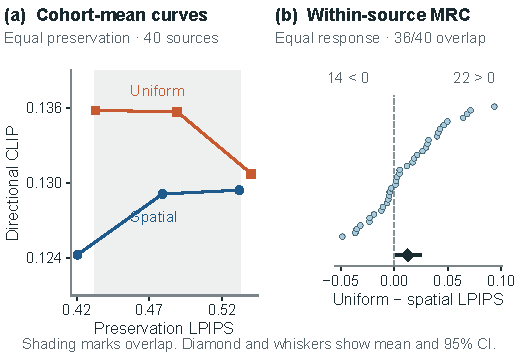
\includegraphics[width=\columnwidth]{figures/v19_aggregation.pdf}
\caption{Source-correction comparisons from three actual settings per arm. (a) Curves connect the three seed- and source-averaged operating points. At common preservation LPIPS the ordinate difference measures directional CLIP. (b) Each point is a source's interval-average preservation LPIPS difference at common directional CLIP, ordered vertically by value. Positive values favor spatial.}
\label{fig:v19-aggregation}\end{figure}
Figure~\ref{fig:v19-aggregation}(a) averages the two seeds and 40 sources for each of the three measured scales per allocation. Over their shared mean LPIPS range [0.43297, 0.53186], uniform minus spatial directional CLIP averages $+0.00652$ [0.00086, 0.01266] (20,000 archived source-bootstrap draws). The cohort-mean directional-CLIP ranges themselves are disjoint: spatial spans [0.12426, 0.12943] and uniform [0.13074, 0.13580].
Panel (b) instead pairs curves within source after averaging the two seeds at each setting. Thirty-six of 40 sources have positive-width directional-CLIP overlap. Of these, 22 favor spatial, 14 favor uniform, and none tie. Uniform minus spatial preservation LPIPS averages $+0.01280$ [0.00219, 0.02396], with median 0.00511. This comparison changes both the matching coordinate and the level at which shared support is constructed.
